\section{Đánh Giá Hiệu Năng}

  \hspace*{0.8cm}Khi so sánh về hiệu năng, Flutter có lợi thế rõ rệt nhờ vào engine render riêng, giúp tối ưu hóa hiệu suất và mang lại trải nghiệm mượt mà, đặc biệt đối với các ứng dụng yêu cầu xử lý đồ họa phức tạp. Flutter thường đạt được tốc độ khung hình ổn định 60 FPS, điều này rất quan trọng đối với những ứng dụng cần hiệu suất cao. Trong khi đó, React Native, mặc dù có thể xử lý tốt với các ứng dụng đơn giản, nhưng đôi khi cần sự can thiệp của các module native để đạt hiệu năng tối ưu. Vì vậy, lựa chọn framework phù hợp phụ thuộc vào yêu cầu hiệu năng cụ thể của dự án.
\vspace{0.5em}

% 4.1
\subsection{Phương Pháp Đánh Giá}
\renewcommand{\labelitemi}{--}    
\subsubsection{Thí Nghiệm 1: Đo FPS Khi Cuộn Danh Sách 1.000 Phần Tử}

  \hspace*{0.8cm}Mục Đích: Đánh giá khả năng xử lý UI phức tạp của các framework khi render danh sách lớn – một tác vụ phổ biến trong ứng dụng di động (mạng xã hội, thương mại điện tử).
\vspace{0.5em}


  \hspace*{0.8cm}\textbf{Thiết Lập Thí Nghiệm:}
  \setlength{\leftmargini}{1.5cm}
  \begin{itemize}
      \item Thiết bị: Xiaomi Redmi Note 10 (Android 12, RAM 4GB).
      \item Công cụ: Android Profiler để đo FPS và Perfetto để phân tích log.
      \item Kịch bản: Tạo danh sách 1.000 phần tử, mỗi phần tử chứa ảnh thumbnail (100x100px), tiêu đề và mô tả.
  \end{itemize}
\vspace{0.5em}

\vspace{0.5em}


  \hspace*{0.8cm}\textbf{Kết Quả:}
\vspace{0.5em}

\begin{figure}[H]
    \centering
    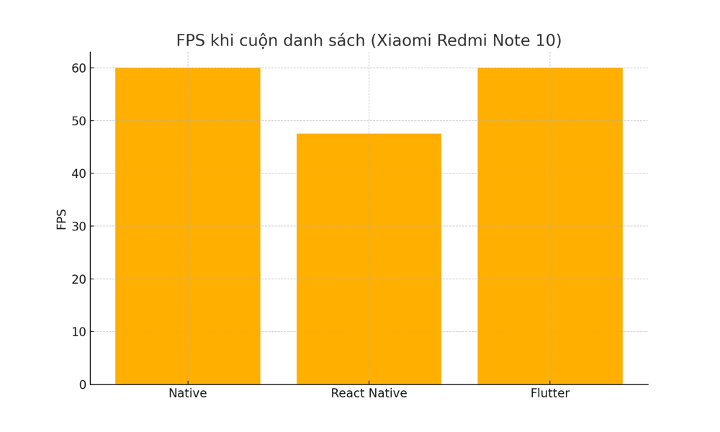
\includegraphics[width=0.85\textwidth]{images/performance_chart.png}
\end{figure}

\vspace{0.5em}

\begin{table}[H]
  \centering
  \begin{tabular}{|l|p{5cm}|p{5cm}|}
  \hline
  \textbf{Framework} & \textbf{FPS Trung Bình} & \textbf{Độ Trễ Tối Đa (ms)} \\
  \hline
  Native       & 60          & 16 \\
  React Native & 45--50      & 35 \\
  Flutter      & 60          & 18 \\
  \hline
  \end{tabular}
  \caption{So sánh FPS và độ trễ tối đa giữa các framework}
  \end{table}
  
  
    \hspace*{0.8cm}Về mặt hiệu suất khung hình, Flutter cho thấy ưu thế nhờ sử dụng Skia Engine để render trực tiếp lên canvas mà không phụ thuộc vào native components. Nhờ đó, Flutter có thể duy trì tốc độ khung hình tối đa 60 FPS một cách ổn định trên hầu hết các thiết bị. Trong khi đó, React Native gặp hạn chế do cơ chế Bridge gây ra độ trễ khi truyền dữ liệu giữa luồng JavaScript và native. Dù React Native đã áp dụng các kỹ thuật tối ưu như VirtualizedList để thực hiện lazy loading, nhưng FPS chỉ cải thiện lên mức tối đa 50, vẫn thấp hơn so với hiệu suất đạt được ở native. Về phía native (sử dụng Kotlin), hệ thống render của Android được tận dụng một cách tối ưu, giúp ứng dụng đạt hiệu suất khung hình ổn định và mượt mà hơn trong hầu hết các kịch bản sử dụng thực tế.
  \vspace{0.5em}
  


  \hspace*{0.8cm}Hạn Chế:
  \setlength{\leftmargini}{1.5cm}
  \begin{itemize}
      \item Thí nghiệm chưa xét đến ảnh hưởng của network request hoặc animation phức tạp.
  \end{itemize}
\vspace{0.5em}

\subsubsection{Thí Nghiệm 2: Đo RAM Sử Dụng}
    
      \hspace*{0.8cm}Mục Đích: So sánh mức tiêu thụ bộ nhớ khi ứng dụng ở trạng thái idle và xử lý tác vụ nặng.
    \vspace{0.5em}

    
      \hspace*{0.8cm}\textbf{Thiết Lập Thí Nghiệm:}
      \setlength{\leftmargini}{1.5cm}
      \begin{itemize}
        \item Ứng dụng mẫu: Xây dựng ứng dụng đọc tin tức với 3 màn hình (danh sách bài viết, chi tiết bài viết, profile).
        \item Công cụ: Android Studio Memory Profiler và Xcode Instruments.
      \end{itemize}
    \vspace{0.5em}
    
    \vspace{0.5em}
    
    
      \hspace*{0.8cm}\textbf{Kết Quả (Trạng Thái Idle):}
    \vspace{0.5em}
    
    \begin{figure}[H]
        \centering
        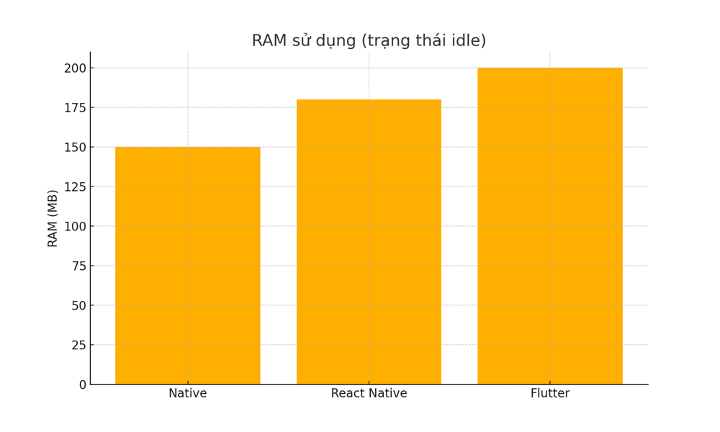
\includegraphics[width=0.75\textwidth]{images/idle_memory_usage.png}
        \caption{So sánh mức sử dụng RAM khi ứng dụng ở trạng thái Idle}
    \end{figure}
    
    \vspace{0.5em}
    
    \begin{table}[H]
      \centering
      \begin{tabular}{|p{5cm}|p{7cm}|}
      \hline
      \textbf{Framework} & \textbf{RAM Sử Dụng (MB)} \\
      \hline
      Native       & 150 \\
      React Native & 180 \\
      Flutter      & 200 \\
      \hline
      \end{tabular}
      \caption{Mức RAM sử dụng trong trạng thái Idle}
  \end{table}
  

  
    \hspace*{0.8cm}Phân Tích:
    Native là giải pháp tiết kiệm RAM nhất vì không cần đến runtime engine phụ trợ. Trong khi đó, React Native tiêu thụ thêm 30MB RAM do JavaScriptCore và Bridge. Flutter, với việc nhúng Dart runtime và Skia Engine, sử dụng nhiều RAM nhất (khoảng 200MB), nhưng sự đánh đổi này giúp cải thiện hiệu suất UI mượt mà hơn.
  \vspace{0.5em}
  
    \hspace*{0.8cm}Kịch Bản Tải Dữ Liệu Nặng: Khi tải 50 ảnh độ phân giải cao (1920x1080px), mức tiêu thụ RAM có sự khác biệt rõ rệt. Flutter tiêu thụ 280MB RAM do việc cache ảnh trong ImageCache. React Native tiêu thụ 250MB RAM nhờ sử dụng FastImage để tối ưu hiệu suất. Trong khi đó, Native chỉ tiêu thụ 210MB RAM nhờ tận dụng Glide cho Android.
  \vspace{0.5em}

  
      \hspace*{0.8cm}Kết Luận: Flutter phù hợp với các thiết bị cao cấp, nhưng có thể tạo ra áp lực đối với các thiết bị giá rẻ. React Native, ngược lại, mang lại sự cân bằng giữa hiệu năng và tài nguyên.
  \vspace{0.5em}

% 4.2
\subsection{Bảng So Sánh Tổng Hợp}
\renewcommand{\labelitemi}{--}    
\begin{table}[H]
  \centering
  \begin{tabular}{|l|c|c|c|c|}
  \hline
  \textbf{Framework} & \textbf{FPS} & \textbf{RAM (MB)} & \textbf{Thời Gian Phát Triển} & \textbf{Hỗ Trợ Nền Tảng} \\
  \hline
  Native       & 60          & 150               & 3 tháng                      & iOS/Android \\
  React Native & 50          & 180               & 1.5 tháng                    & iOS/Android/Web \\
  Flutter      & 60          & 200               & 2 tháng                      & iOS/Android/Web/Desktop \\
  \hline
  \end{tabular}
  \caption{So sánh các framework về FPS, RAM, Thời gian phát triển và Hỗ trợ nền tảng}
  \end{table}
  

  
      \hspace*{0.8cm}FPS: Native và Flutter đều đạt 60 FPS nhờ vào việc tối ưu render engine. Tuy nhiên, React Native chỉ đạt giới hạn 50 FPS do giao tiếp qua Bridge, dẫn đến một sự chậm trễ trong quá trình render.
  \vspace{0.5em}

  
      \hspace*{0.8cm}RAM: Native là giải pháp tiết kiệm RAM nhất, trong khi Flutter tiêu thụ RAM nhiều nhất do kiến trúc tự render, yêu cầu nhiều tài nguyên hơn để duy trì hiệu suất.
  \vspace{0.5em}

  
      \hspace*{0.8cm}Thời Gian Phát Triển: React Native giúp giảm 50\% thời gian phát triển nhờ khả năng tái sử dụng code từ các dự án web. Ngược lại, Flutter yêu cầu thời gian học thêm Dart và hiểu rõ về widget tree để làm việc hiệu quả với framework này.
  \vspace{0.5em}

% 4.3
\subsection{Thảo Luận}
\renewcommand{\labelitemi}{--}    
\subsubsection{Flutter: Lựa Chọn Cho Ứng Dụng Đồ Họa Cao}

  \hspace*{0.8cm}Flutter phù hợp với các dự án yêu cầu UI tùy chỉnh cao và animation phức tạp nhờ:
  \setlength{\leftmargini}{1.5cm}
  \begin{itemize}
    \item Skia Engine: Render mượt mà, hỗ trợ hiệu ứng như blur, gradient, và transform 3D.
    \item AOT Compilation: Tối ưu hiệu năng cho thiết bị đa dạng.
  \end{itemize}
\vspace{0.5em}


  \hspace*{0.8cm}Ví Dụ Thực Tế:
  \setlength{\leftmargini}{1.5cm}
  \begin{itemize}
      \item Ứng dụng Reflectly (nhật ký cá nhân): Sử dụng Flutter để tạo animation chuyển cảnh mượt, đạt 60 FPS trên iPhone SE (2020).
      \item Game 2D đơn giản: Flutter xử lý tốt physics engine và particle effects.
  \end{itemize}
\vspace{0.5em}


  \hspace*{0.8cm}Hạn Chế:
  \setlength{\leftmargini}{1.5cm}
  \begin{itemize}
      \item Kích thước ứng dụng lớn: Khó triển khai ở thị trường có hạ tầng Internet kém (ví dụ: Đông Nam Á).
      \item Tài nguyên phần cứng: tiêu thụ RAM cao gây lag trên các thiết bị cũ (RAM $\leq$ 2GB).
  \end{itemize}
\vspace{0.5em}

\subsubsection{React Native: Tối Ưu Cho MVP Và Ứng Dụng Doanh Nghiệp}
    
      \hspace*{0.8cm}React Native phù hợp với các dự án cần triển khai nhanh và tích hợp hệ thống sẵn có:
      \setlength{\leftmargini}{1.5cm}
      \begin{itemize}
        \item Tái Sử Dụng Code Web: Giảm chi phí phát triển, phù hợp startup. Ví dụ: Ứng dụng Delivery Foodcủa Grab tái sử dụng 70\% code từ web.
        \item Hỗ Trợ Module Native: Dễ dàng tích hợp SDK thanh toán (Visa, Mastercard) hoặc xác thực (Firebase Auth).
      \end{itemize}
    \vspace{0.5em}

    
      \hspace*{0.8cm}Ví Dụ Thực Tế:
      \setlength{\leftmargini}{1.5cm}
      \begin{itemize}
          \item Ứng dụng Bloomberg: Sử dụng React Native để đồng bộ dữ liệu chứng khoán real-time giữa web và mobile.
          \item Doanh Nghiệp: Walmart, Microsoft Teams sử dụng React Native để duy trì codebase chung.
      \end{itemize}
    \vspace{0.5em}

    
      \hspace*{0.8cm}Hạn Chế:
      \setlength{\leftmargini}{1.5cm}
      \begin{itemize}
          \item Hiệu Năng: Không phù hợp ứng dụng xử lý ảnh/video thời gian thực
          \item Phụ Thuộc Thư Viện: Cập nhật phiên bản thường xuyên để tránh lỗi bảo mật.
      \end{itemize}
    \vspace{0.5em}

    \subsubsection{Native: Giải Pháp Tối Ưu Cho Ứng Dụng Chuyên Sâu}
    
      \hspace*{0.8cm}Native (Kotlin/Swift) vẫn là lựa chọn hàng đầu cho:
      \setlength{\leftmargini}{1.5cm}
      \begin{itemize}
        \item Ứng dụng yêu cầu phần cứng: AR/VR (ARKit, ARCore), xử lý AI trên thiết bị (Core ML).
        \item Dự Án Lớn: Ngân hàng, y tế – nơi cần tối ưu bảo mật và hiệu năng.
      \end{itemize}
    \vspace{0.5em}

    
      \hspace*{0.8cm}Ví Dụ:
      \setlength{\leftmargini}{1.5cm}
      \begin{itemize}
          \item Instagram: Chuyển sang native code cho tính năng Reels để đạt độ trễ dưới 50ms.
          \item Ứng dụng Ngân Hàng: Techcombank sử dụng native để xử lý giao dịch an toàn.
      \end{itemize}
    \vspace{0.5em}

% 4.4
\subsection{Kết Luận}
\renewcommand{\labelitemi}{--}    

  \hspace*{0.8cm}Việc lựa chọn framework phụ thuộc vào mục tiêu dự án và nguồn lực:
  \setlength{\leftmargini}{1.5cm}
  \begin{itemize}
      \item Flutter: Ưu tiên UI/UX và đa nền tảng.
      \item React Native: Tập trung MVP và tích hợp hệ sinh thái web.
      \item Native: Phát triển ứng dụng chuyên sâu, tận dụng tối đa phần cứng.
  \end{itemize}
\vspace{0.5em}


  \hspace*{0.8cm}Xu Hướng 2024:
  \setlength{\leftmargini}{1.5cm}
  \begin{itemize}
      \item Flutter cải thiện kích thước ứng dụng với Impeller Engine (thay Skia).
      \item React Native tăng tốc độ render qua Fabric và TurboModules.
  \end{itemize}
\vspace{0.5em}